
%%% Template originaly created by Karol Kozioł (mail@karol-koziol.net) and modified for ShareLaTeX use

\documentclass[a4paper,11pt]{article}

\usepackage{amsmath}
\usepackage[T1]{fontenc}
\usepackage[utf8]{inputenc}
\usepackage{graphicx}
\usepackage[usenames,dvipsnames]{xcolor}

\usepackage{sansmath}
\renewcommand\familydefault{\sfdefault}
\usepackage{tgheros}

\usepackage{amsmath,amssymb,amsthm,textcomp}
\usepackage{enumerate}
\usepackage{multicol}
\usepackage{tikz}
\usetikzlibrary{shapes, positioning}

\usepackage[super]{nth}
\usepackage{wrapfig}

\usepackage{geometry}
\geometry{total={210mm,297mm},
left=25mm,right=25mm,%
bindingoffset=0mm, top=20mm,bottom=20mm}


\linespread{1.3}

\newcommand{\linia}{\rule{\linewidth}{0.5pt}}

% custom theorems if needed
\newtheoremstyle{mytheor}
    {1ex}{1ex}{\normalfont}{0pt}{\scshape}{.}{1ex}
    {{\thmname{#1 }}{\thmnumber{#2}}{\thmnote{ (#3)}}}

\theoremstyle{mytheor}
\newtheorem{defi}{Definition}

% my own titles
\makeatletter
\renewcommand{\maketitle}{
\begin{center}
\vspace{2ex}
{\huge \textsc{\@title}}
\vspace{1ex}
\\
\linia\\
\@author \hfill \@date
\vspace{4ex}
\end{center}
}
\makeatother
%%%

% custom footers and headers
\usepackage{fancyhdr}
\pagestyle{fancy}
\lhead{}
\chead{}
\rhead{}
\lfoot{Automatic~Verification Assignment \#4}
\cfoot{}
\rfoot{Page \thepage}
\renewcommand{\headrulewidth}{0pt}
\renewcommand{\footrulewidth}{0pt}
%

% all section titles centered and bolded
\usepackage{sectsty}
\allsectionsfont{\bfseries\large}
%
% add section label
\renewcommand\thesection{Problem~\arabic{section}:}
\renewcommand\thesubsection{(\alph{subsection})}
%

%%%----------%%%----------%%%----------%%%----------%%%

\begin{document}

\title{Homework Assignment~\#4}

\author{R02943142 Hsieh, Chiao}

\maketitle

\section{$\mu$-Calculus}
Consider an extended Kripke structure $M$ as shown below:

\begin{center}
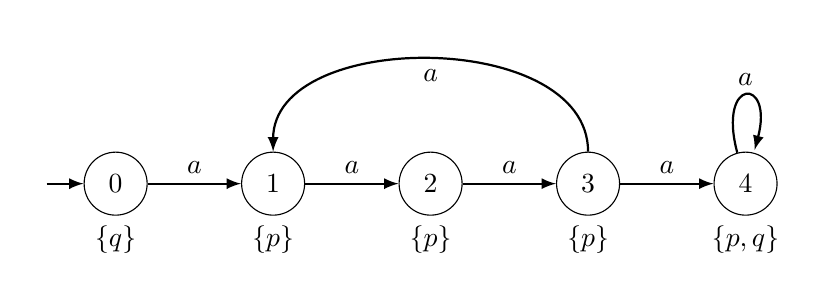
\begin{tikzpicture}[
  scale=2,
  state/.style = {draw, circle, minimum width=8mm, minimum height=8mm},
  every edge/.style = {draw, ->, >=latex, thick},
  trans/.style = {edge label = $a$}
]
  \node (i) at (-0.5, 0){};
  \node[state][label={below:$\{q\}$}]
    (0) at (0, 0) {$0$};
  \node[state][label={below:$\{p\}$}]
    (1) at (1, 0) {$1$};
  \node[state][label={below:$\{p\}$}]
    (2) at (2, 0) {$2$};
  \node[state][label={below:$\{p\}$}]
    (3) at (3, 0) {$3$};
  \node[state][label={below:$\{p,q\}$}]
    (4) at (4, 0) {$4$};

  \path
    (i) edge (0)
    (0) edge[trans] (1)
    (1) edge[trans] (2)
    (2) edge[trans] (3)
    (3) edge[trans] (4)
    
    (3) edge[trans,bend right=90] (1)
    (4) edge[trans,loop above] (4)
  ;
\end{tikzpicture}
\end{center}
Show the iterative valuations and the final result for the following fixpoints in $\mu$-calculus:

\newcommand{\Eval}{\texttt{Eval}}
\newcommand{\Evalp}{\{1,2,3,4\}}
\newcommand{\Evalq}{\{0,4\}}


\subsection{$\mu Q.(q \vee (p \wedge \langle a \rangle Q))$}
Answer.
\smallskip \\
To compute the fixpoint, we follow the \texttt{Eval} procedure and find $\Eval(\mu Q.(q \vee (p \wedge \langle a \rangle Q)), e)$. Here we present the result of each iteration of fixpoint computation in bottom-up manner.

\noindent \textbf{Atomic Propositions:}
\[
\begin{array}{ll}
  \Eval(q, e) = \Evalq &\qquad \Eval(p, e) = \Evalp \\
\end{array}
\]
\textbf{\nth{0} Iteration:} 
\(Q_{old} \gets \bot,\quad e'\gets e[Q \gets Q_{old}]\)
\[
\arraycolsep=1.4pt
\begin{array}{ll}
  \Eval(Q, e') 
    &= e[Q \gets Q_{old}](Q) = Q_{old} = \bot \\
  \Eval(\langle a \rangle Q, e') 
    &= \{s \mid \exists t. s \xrightarrow{a} t \wedge t \in \Eval(Q, e')\} \\
    &= \{s \mid \exists t. s \xrightarrow{a} t \wedge t \in \bot\} = \bot\\
  Q_{val}
    &= \Eval((q \vee (p \wedge \langle a \rangle Q)), e')\\
    &= \Eval(q, e') \cup (\Eval(p,e') \cap \Eval(\langle a \rangle Q,e')) \\
    &= \Evalq \cup (\Evalp \cap \bot)=\{0,4\} \\
    &\neq Q_{old}
\end{array}
\]
\textbf{\nth{1} Iteration:} 
\(Q_{old} \gets \{0,4\},\quad e'\gets e[Q \gets Q_{old}]\)
\[
\arraycolsep=1.4pt
\begin{array}{ll}
  \Eval(Q, e') 
    &= \{0,4\} \\
  \Eval(\langle a \rangle Q, e') 
    &= \{s \mid \exists t. s \xrightarrow{a} t \wedge t \in \{0,4\}\} \\
    &= \{3,4\} \\
  Q_{val}
    &= \Evalq \cup (\Evalp \cap \{3,4\})=\{0,3,4\} \\
    &\neq Q_{old}
\end{array}
\]
\textbf{\nth{2} Iteration:} 
\(Q_{old} \gets \{0,3,4\},\quad e'\gets e[Q \gets Q_{old}]\)
\[
\arraycolsep=1.4pt
\begin{array}{ll}
  \Eval(Q, e') 
    &= \{0,3,4\} \\
  \Eval(\langle a \rangle Q, e') 
    &= \{s \mid \exists t. s \xrightarrow{a} t \wedge t \in \{0,3,4\}\} \\
    &= \{2,3,4\} \\
  Q_{val}
    &= \Evalq \cup (\Evalp \cap \{2,3,4\}) =\{0,2,3,4\} \\
    &\neq Q_{old}
\end{array}
\]
\textbf{\nth{3} Iteration:} 
\(Q_{old} \gets \{0,2,3,4\},\quad e'\gets e[Q \gets Q_{old}]\)
\[
\arraycolsep=1.4pt
\begin{array}{ll}
  \Eval(Q, e') 
    &= \{0,2,3,4\} \\
  \Eval(\langle a \rangle Q, e') 
    &= \{s \mid \exists t. s \xrightarrow{a} t \wedge t \in \{0,2,3,4\}\} \\
    &= \{1,2,3,4\} \\
  Q_{val}
    &= \Evalq \cup (\Evalp \cap \{1,2,3,4\}) =\{0,1,2,3,4\} \\
    &\neq Q_{old}
\end{array}
\]
\textbf{\nth{4} Iteration:} 
\(Q_{old} \gets \{0,1,2,3,4\},\quad e'\gets e[Q \gets Q_{old}]\)
\[
\arraycolsep=1.4pt
\begin{array}{ll}
  \Eval(Q, e') 
    &= \{0,1,2,3,4\} \\
  \Eval(\langle a \rangle Q, e') 
    &= \{s \mid \exists t. s \xrightarrow{a} t \wedge t \in \{0,1,2,3,4\}\} \\
    &= \{0,1,2,3,4\} \\
  Q_{val}
    &= \Evalq \cup (\Evalp \cap \{0,1,2,3,4\}) =\{0,1,2,3,4\} \\
    &= Q_{old}
\end{array}
\]
Hence, the least fixpoint is \(\{0,1,2,3,4\}\).

\subsection{$\mu Q_1.(\nu Q_2.(p \wedge \langle a \rangle Q_2) \vee (q \wedge \langle a \rangle Q_1))$}
Answer.
\smallskip \\
\textbf{Iteration 00:} 
\(
  Q_1^0 \gets \bot,\quad Q_2^{00} \gets \top,\quad
  e' \gets e[Q_1 \gets Q_1^0; Q_2 \gets Q_2^{00}] 
\)
\[
\arraycolsep=1.4pt
\begin{array}{ll}
  \Eval&(\langle a \rangle Q_1, e') = \bot
    \qquad \Eval(\langle a \rangle Q_2, e') = \top \\
  Q_2^{01}
    &= (\Evalp \cap \top) \cup (\Evalq \cap \bot)\\
    &= \{1,2,3,4\} \\
    &\neq Q_2^{00}
\end{array}
\]
\textbf{Iteration 01:} 
\(
  Q_1^0 \gets \bot,\quad Q_2^{01} \gets \{1,2,3,4\},\quad
  e' \gets e[Q_1 \gets Q_1^0; Q_2 \gets Q_2^{01}] 
\)
\[
\arraycolsep=1.4pt
\begin{array}{ll}
  \Eval&(\langle a \rangle Q_1, e') = \bot
    \qquad \Eval(\langle a \rangle Q_2, e') = \top \\
  Q_2^{02}
    &= (\Evalp \cap \top) \cup (\Evalq \cap \bot)\\
    &= \{1,2,3,4\} \\
    &= Q_2^{01} \qquad\text{Found fixpoint for } Q_2\\
  Q_1^1
    &= \Eval(\nu Q_2.(p \wedge \langle a \rangle Q_2) \vee (q \wedge \langle a \rangle Q_1), e') = Q_2^{01} \\
    &= \{1,2,3,4\} \\
    &\neq Q_1^0
\end{array}
\]
\textbf{Iteration 10:} 
\(
  Q_1^1 \gets \{1,2,3,4\},\quad Q_2^{10} \gets \top,\quad
  e' \gets e[Q_1 \gets Q_1^1; Q_2 \gets Q_2^{10}] 
\)
\[
\arraycolsep=1.4pt
\begin{array}{ll}
  \Eval&(\langle a \rangle Q_1, e') = \top
    \qquad \Eval(\langle a \rangle Q_2, e') = \top \\
  Q_2^{11}
    &= (\Evalp \cap \top) \cup (\Evalq \cap \top)\\
    &= \{0,1,2,3,4\} = \top\\
    &= Q_2^{10} \qquad\text{ Found fixpoint for } Q_2\\
  Q_1^2
    &= Q_2^{10} = \top \\
    &\neq Q_1^1
\end{array}
\]
\textbf{Iteration 20:} 
\(
  Q_1^2 \gets \top,\quad Q_2^{20} \gets \top,\quad
  e' \gets e[Q_1 \gets Q_1^2; Q_2 \gets Q_2^{20}] 
\)
\[
\arraycolsep=1.4pt
\begin{array}{ll}
  \Eval&(\langle a \rangle Q_1, e') = \top
    \qquad \Eval(\langle a \rangle Q_2, e') = \top \\
  Q_2^{21}
    &= (\Evalp \cap \top) \cup (\Evalq \cap \top)\\
    &= \{0,1,2,3,4\} = \top\\
    &= Q_2^{20} \qquad\text{ Found fixpoint for } Q_2\\
  Q_1^3
    &= Q_2^{20} = \top \\
    &= Q_1^2 \qquad\text{ Found fixpoint for } Q_1\\
\end{array}
\]
Hence, the least fixpoint is \(\{0,1,2,3,4\}\).

\section{NuSMV}
The following is a NuSMV model for two asynchronous processes 
that use a semaphore to achieve mutual exclusion.
\begin{verbatim}
MODULE main
VAR
  semaphore : boolean;
  proc1 : process user(semaphore);
  proc2 : process user(semaphore);
ASSIGN
  init(semaphore) := 0;

MODULE user(semaphore)
VAR
  state : {idle, entering, critical, exiting};
ASSIGN
  init(state) := idle;
  next(state) :=
  case
    state = idle : {idle, entering};
    state = entering & !semaphore : critical;
    state = critical : {critical, exiting};
    state = exiting : idle;
    1 : state;
  esac;
next(semaphore) :=
  case
    state = entering : 1;
    state = exiting : 0;
    1 : semaphore;
  esac;
\end{verbatim}



\subsection{Write all the necessary boolean formulae that
specify the main module as a Kripke structure; you may define
shorter substitute names for the variables to save space.}
Answer.
\smallskip \\
For simple representation with boolean formulae, we use $sem$ to denote \texttt{semaphore} and also encode \texttt{state} using two boolean variables $s_0,s_1$ with following mapping on each value of \texttt{state}.
\[
\begin{array}{lcl}
  \texttt{state}=\texttt{idle} & \Leftrightarrow & (s_0,s_1)=(0,0) \text{ or } \neg{s_0}\neg{s_1} \text{ for short}\\
  \texttt{state}=\texttt{entering} & \Leftrightarrow & \neg{s_0}s_1 \\
  \texttt{state}=\texttt{critical} & \Leftrightarrow & s_0s_1 \\ 
  \texttt{state}=\texttt{exiting} & \Leftrightarrow & s_0\neg{s_1} \\
 && 
\end{array}
\]
Also we use superscript to distinguish the scope of the 
variables. For example, $s_1^{1}$ means this variable is for process \texttt{proc1}. If there is no superscript on the variable, it is a global variable.
With these notations, the construction for one process is 
straight forward. Following is the construction for \texttt{proc1}. Model for \texttt{proc2} can be constructed in the same way only with different superscript.
\[
\arraycolsep=1.4pt
\begin{array}{lcll}
  \multicolumn{3}{c}{M^\texttt{proc1} = (S^1,I^1,R^1,L^1)}  \\
  I^1 &=& \neg{s_0^1}\neg{s_1^1} &\texttt{\% idle} \\
  R^1 &=&\neg{s_0^1}\neg{s_1^1}(\neg{s_0^1}'\neg{s_1^1}' + \neg{s_0^1}'{s_1^1}')
         &\texttt{\% idle :\ \{idle, entering\}} \\
      &+& \neg{s_0^1}{s_1^1}(\neg{sem}){s_0^1}'{s_1^1}'
         &\texttt{\% entering \& !semaphore :\ critical} \\
      &+& {s_0^1}{s_1^1}({s_0^1}'{s_1^1}'+{s_0^1}'\neg{s_1^1}')
         &\texttt{\% critical :\ \{critical, exiting\}} \\
      &+& {s_0^1}\neg{s_1^1}{\neg{s_0^1}'\neg{s_1^1}'
         &\texttt{\% exiting :\ idle} \\
      &+& (s_0^1 \equiv {s_0^1}')(s_1^1 \equiv {s_1^1}')
         &\texttt{\% 1 :\ state} \\
      &+& \neg{s_0^1}{s_1^1}(sem') &\texttt{\% entering :\ 1} \\
      &+& {s_0^1}\neg{s_1^1}(\neg{sem'}) 
         &\texttt{\% exiting :\ 0} \\
      &+& (sem \equiv sem') &\texttt{\% 1 :\ semaphore} \\
\end{array}
\]
To compute the Kripke structure for the main module, we have to compose \texttt{proc1} and \texttt{proc2} with interleaving. Formally,
\[
\begin{array}{ll}
  \multicolumn{2}{c}{M^\texttt{main} = (S,I,R,L)}\\
  I &= \neg{sem} \cdot I^1 \cdot I^2 = (\neg{sem})\neg{s_0^1}\neg{s_1^1}\neg{s_0^2}\neg{s_1^2} \\
  R &= R^1 \cdot R^2 \\
\end{array}
\]

\subsection{Please draw BDD diagrams (as small as possible) for
the formulae in 2a.}
Answer. The variable order for both BDDs is 
$(s_0^1, s_1^1, {s_0^1}', {s_1^1}',s_0^2, s_1^2, {s_0^2}', {s_1^2}', sem, sem')$.

\begin{wrapfigure}{l}{\textwidth}
\centering
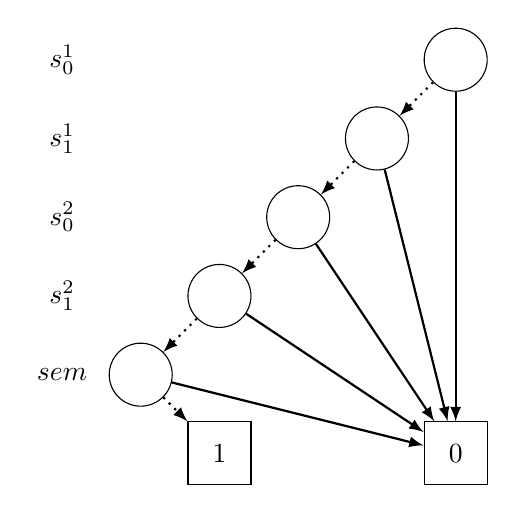
\begin{tikzpicture}[
  scale=1,
  every node/.style = {minimum width=8mm, minimum height=8mm},
  state/.style = {draw, circle},
  const/.style = {draw, rectangle},
  every edge/.style = {draw, ->, >=latex, thick},
  edge1/.style = {},
  edge0/.style = {dotted}
]
  \node (v1) at (0, 5) {$s_0^1$};
  \node (v2) at (0, 4) {$s_1^1$};
  \node (v3) at (0, 3) {$s_0^2$};
  \node (v4) at (0, 2) {$s_1^2$};
  \node (v0) at (0, 1) {$sem$};

  \node[state] (n0) at (5, 5) {};
  \node[state] (n1) at (4, 4) {};
  \node[state] (n2) at (3, 3) {};
  \node[state] (n3) at (2, 2) {};
  \node[state] (n4) at (1, 1) {};
  
  \node[const] (1)  at (2, 0) {$1$};
  \node[const] (0)  at (5, 0) {$0$};

  \path
    (n0) edge[edge0] (n1)
         edge[edge1] (0)
    (n1) edge[edge0] (n2)
         edge[edge1] (0)
    (n2) edge[edge0] (n3)
         edge[edge1] (0)
    (n3) edge[edge0] (n4)
         edge[edge1] (0)
    (n4) edge[edge0] (1)
         edge[edge1] (0)
  ;
\end{tikzpicture}
\caption{BDD for Initial States $I$}
\label{fig:BDD_I}
\end{wrapfigure}

\begin{wrapfigure}{l}{\textwidth}
\centering
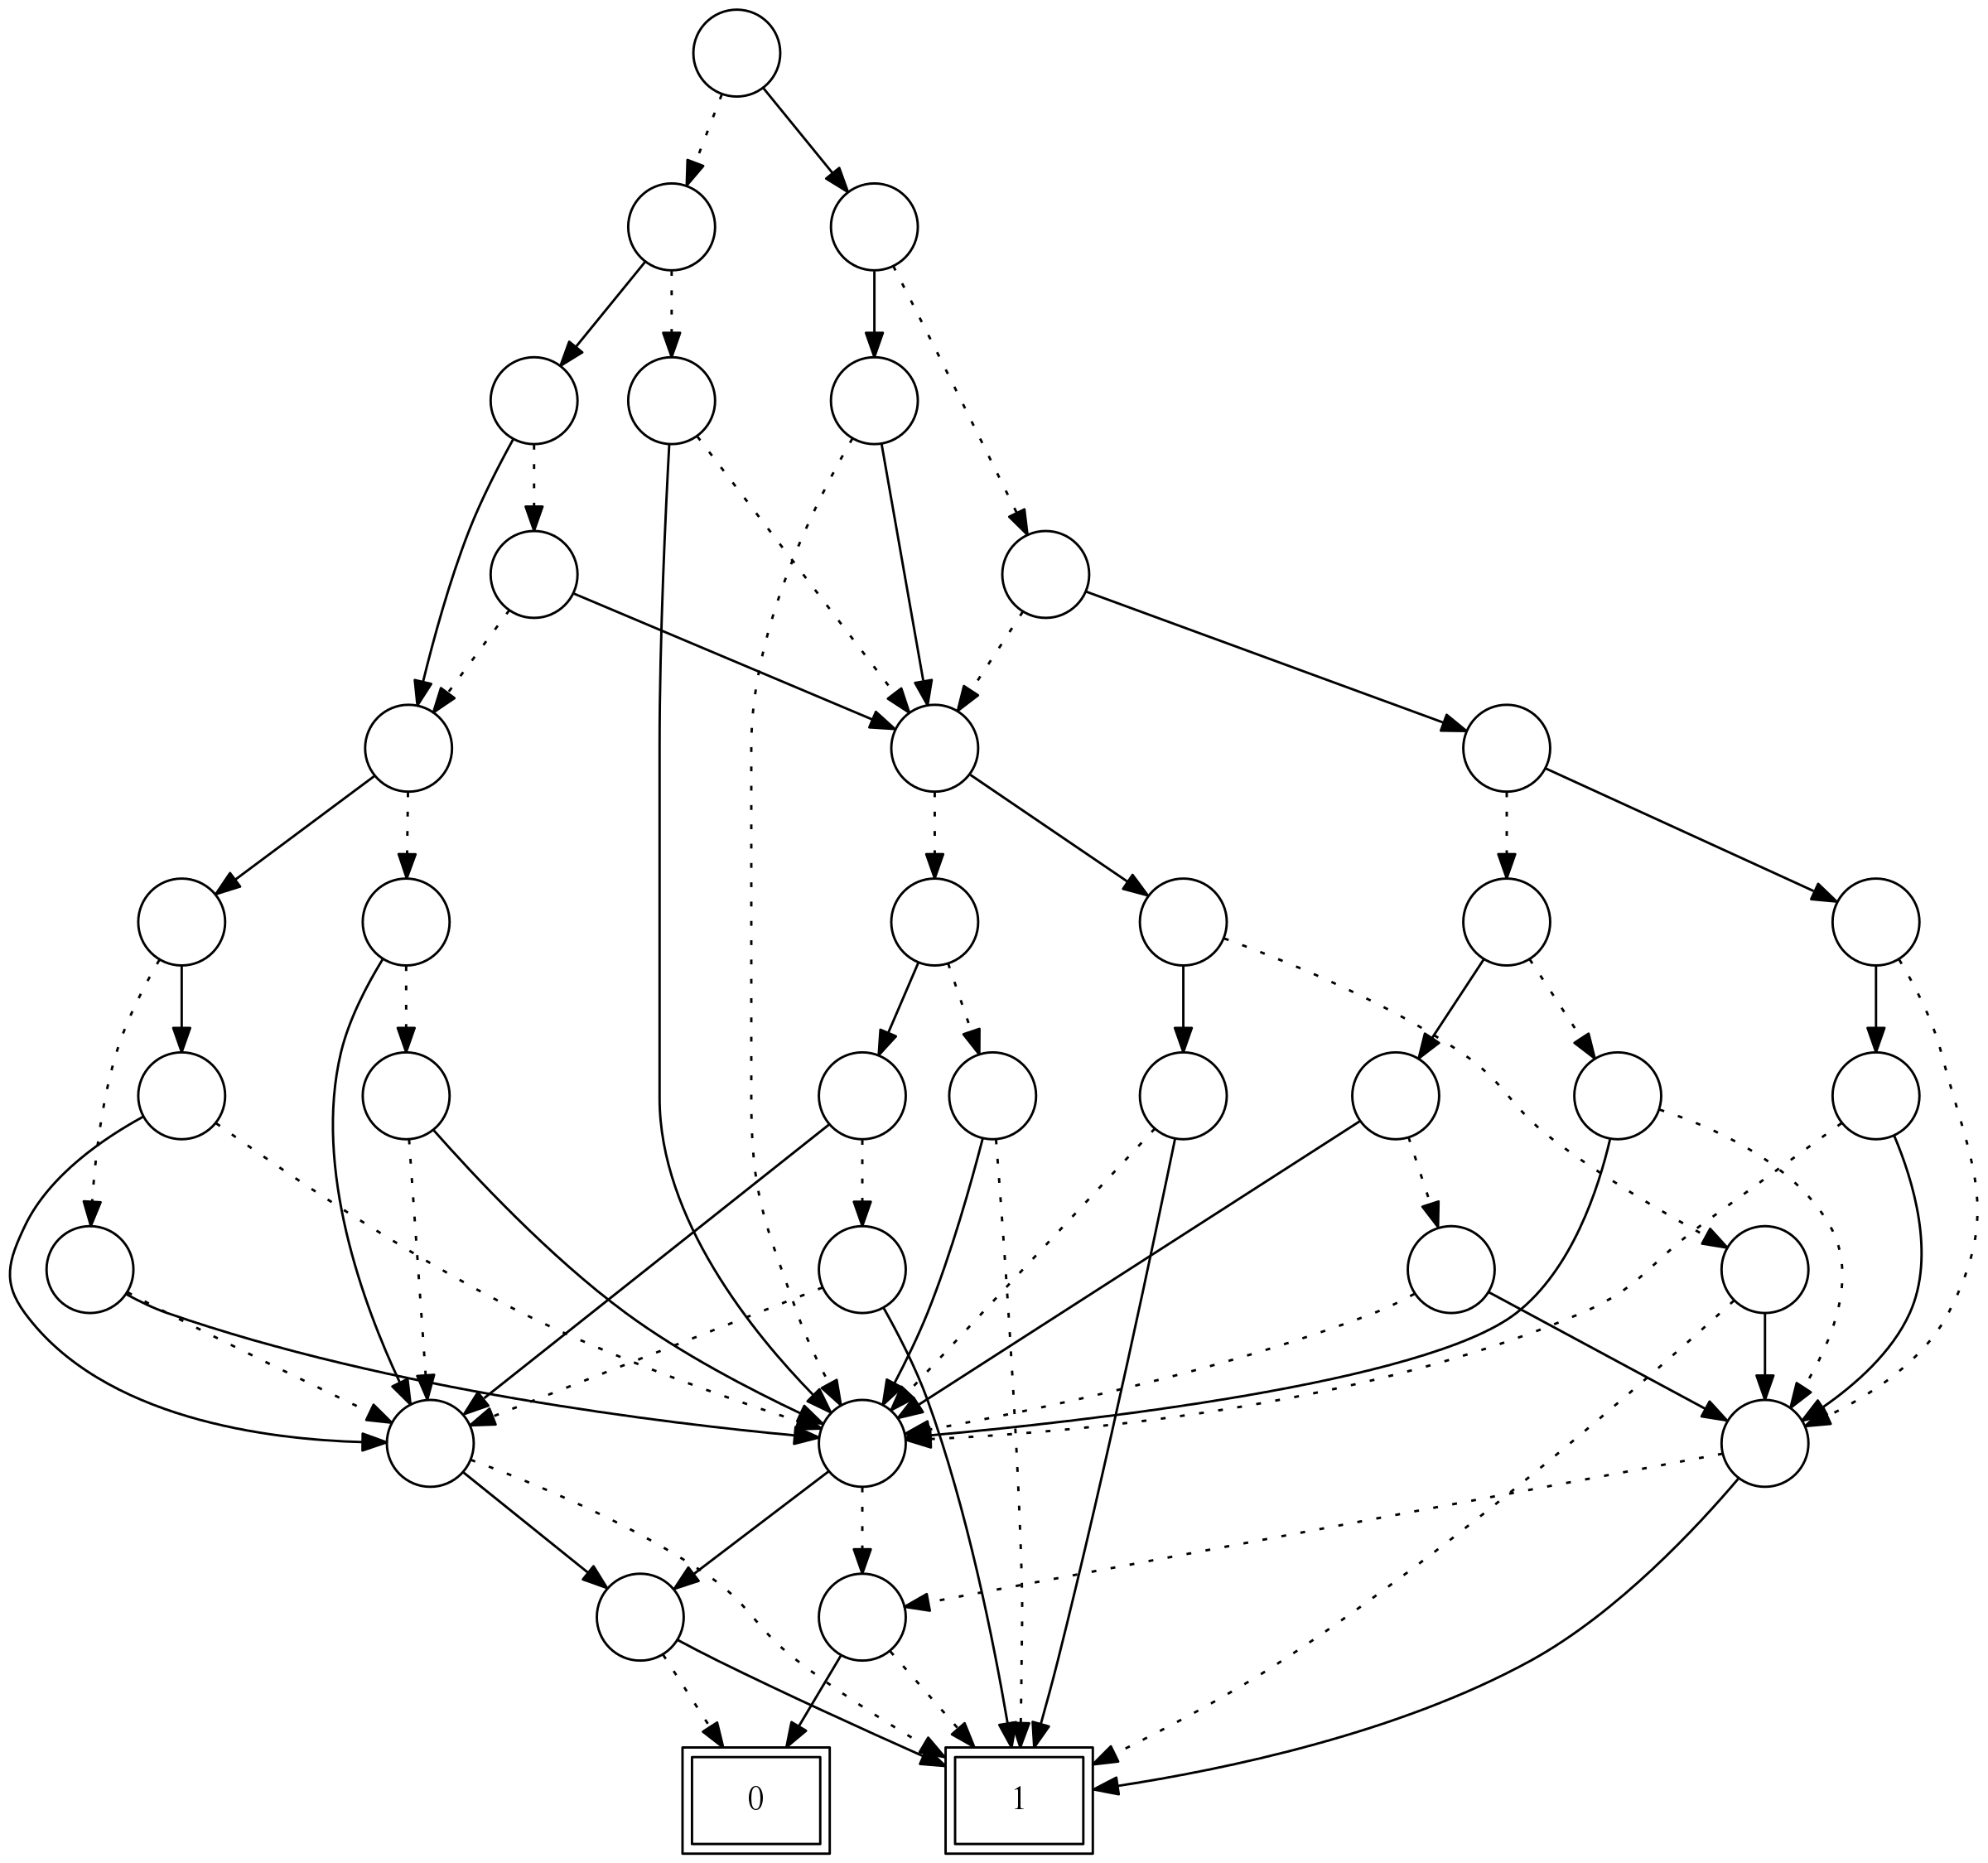
\includegraphics[width=\textwidth]{HW4_bdd}
\caption{BDD for Transition Relation $R$}
\label{fig:BDD_R}
\end{wrapfigure}


\end{document}
